%Chapter 3

\renewcommand{\thechapter}{3}

\chapter{Automated Classification for Diffraction Image Data}

\section{Overview}
In this research, we apply the supervised learning algorithm in machine learning to support automated classification of images. In general, supervised learning conducts a model using a set of labeled training examples\cite{Mehryar}. Each example is a pair including an object as input and desired value as output. Typically, the input object is represented by an M-by-N matrix where M is the number of training examples and N is the number of feature parameters in an example and the desired output value is called the supervisory signal. Thus, we construct the feature vector using the texture features calculated from GLCM and assign the desired output with diffraction image type which is cell, debris or strip. To realize supervised learning, there are lots of approaches and algorithms which are proposed and developed, such as support vector machine (SVM)\cite{Cortes}, artificial neural network\cite{McCulloch}, and so on.

\section{Support Vector Machine Algorithm}
SVM is a supervised learning model in machine learning for classification and regression analysis\cite{Cortes}. Given a set of labeled training data, the algorithm generates an optimal model which can be used to classify new examples. Given a set of training data of the form \{($x_1,y_1$),($x_2,y_2$),\ldots,($x_N,y_N$)\} where N is the number of examples in the training data set, the major purpose of the SVM algorithm is to create a function 
\textit{f :} X $\rightarrow$ Y,
where $x_i$ $\in$ X (\textit{i} = 1,2,3,\ldots,N) is a training example with different feature parameters of an object and $y_i$ $\in$ Y is the output value corresponding to the $x_i$. For instance, the value of $y_i$ is sometimes either +1 or -1 for classification problem.   
\par
In SVM, the primary step is to achieve the hypothesis representation defined as 
\begin{equation}
    h_\theta(x) = \theta _0 + \theta_1x_1 + \theta_2x_2 + \theta_3x_3 + \dots + \theta_nx_n 
\end{equation}
where $x_n$ is the value of $n^{th}$ feature parameter in the training example. By considering the definition of matrix multiplication, the hypothesis representation also can be represented as 
\begin{equation}
    h_\theta(x) = 
    \begin{bmatrix}
        \theta_0 & \theta_1 & \dots & \theta_n
    \end{bmatrix}
    \begin{bmatrix}
        x_0\\
        x_1\\
        \vdots\\
        x_n
    \end{bmatrix}
    = \theta^Tx
\end{equation}
where $x_0$ normally equals 1 from a computation perspective. Once we achieve the hypothesis function, we can translate the output of the hypothesis function as follows
\begin{equation}
     y=\left\{
  \begin{array}{@{}ll@{}}
    1, & \text{if}\ h_\theta(x) \geq 1 \\
    -1, & \text{if}\ h_\theta(x) \leq -1
  \end{array}\right.
\end{equation}
to get the discrete -1 or 1 classification. Due to the circumstances, the line that separates the area where y = 1 and where y = -1 is called the decision boundary. Figure 3.1 is an instance of the decision boundary. Taking spam classification for email as an example, we create a set of training examples by converting each email into a feature vector $x \in R^n$ by referring to the vocabulary list. For this example, n is the number of words in vocabulary list, and the feature $x_i\in {0,1}$ for an email depends on whether or not the $i^{th}$ word appears in the email. Given the label y $\in \{1, -1\}$, the corresponding feature vector looks like this: 
\begin{figure}[!b]
    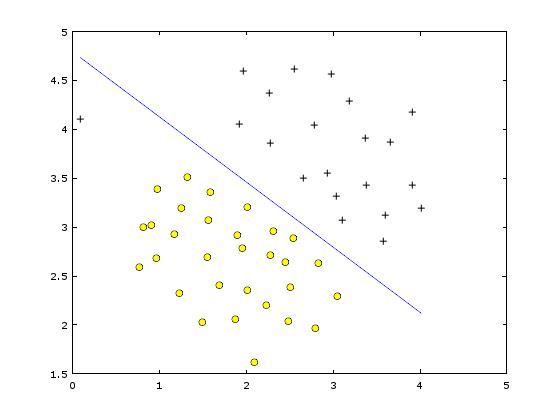
\includegraphics[width = \linewidth]{Fig1}
    \caption{A decision boundary that separates two class areas}
    \label{fig3.1}
\end{figure}
\begin{align*}
x = 
\renewcommand{\arraystretch}{0.4}
\begin{bmatrix}
        & 0 &\\
        & \vdots &\\
        & 1 &\\
        & 0 &\\
        & \vdots &\\
        & 0 &\\
        & 1 &\\
        & \vdots &\\
        & 0 &
    \end{bmatrix}
    \in R^n
\end{align*}
By training the SVM classifier on multiple data like this, we can achieve a model which is able to predict a new example of either the spam-email or the nonspam-email.\par   
However, the decision boundary may not be a linear line most of the time. In order to solve more complex and non-linear classification problems, the kernel method is proposed in SVM to create the corresponding classifier. Given training set ($x^{(1)}$, $y^{(1)}$), ($x^{(2)}$, $y^{(2)}$), \ldots, ($x^{(m)}$, $y^{(m)}$), we choose 
\begin{align*}
    l^{(1)} = x^{(1)}, l^{(2)} = x^{(2)}, \ldots, l^{(m)} = x^{(m)}
\end{align*}
Due to the circumstances, an example x is given so that we can have
\begin{align*}
    f_1 = similarity(x, l^{(1)})\\
    f_2 = similarity(x, l^{(2)})\\
    \dots 
\end{align*}
As a result, we can build a map as follows
\begin{align*}
    g: x^{(i)} \rightarrow 
    \begin{bmatrix}
        f_1^{(i)} \\
        f_2^{(i)} \\
        \dots \\
        f_m^{(i)} \\
    \end{bmatrix}
\end{align*}
where $f_i^{(i)}$ = similarity($x^{(i)}$, $l^{(i)}$) = K($x^{(i)}$, $l^{(i)}$) that is the representation of the kernel.\par
In addition, the SVM algorithm can be applied in not only binary classification, but also multiple-class classification. To solve multiple-class classification problems, a common approach called one-vs-all is introduced. The one-vs-all approach is evolved from the binary classification approach by considering the fact that the multiple-class classification problem can be considered as an n+1 binary classification problem. For example, we can assume that we have a set of class data y $\in$ \{0, 1, 2, $\ldots$, n\} where n means the number of classes in the data. By considering it as an n+1 binary classification problem, we can select one class and then group all the others into a single second class. We predict the probability of each selecting class through the formula as follows:
\begin{align*}
    {h_\theta}^{(0)}(x) = P (y = 0 | x ;\theta)\\
    {h_\theta}^{(1)}(x) = P (y = 1 | x ;\theta)\\
    \ldots \ldots \ldots \ldots\\
    {h_\theta}^{(n)}(x) = P (y = n | x ;\theta)
\end{align*}
Eventually, after repeating the process for all classes, we can achieve the highest value as a prediction by using the hypothesis as follows:
\begin{align*}
    prediction = max ({h_\theta}^{(i)}(x))
\end{align*}
As a result, the SVM algorithm can solve the classification problem with more than two classes via the one-vs-all approach.

\section{The Integrated Tool for SVM Classifier}
LIBSVM is a very useful integrated software for SVM algorithm\cite{Chang}. There are four basic kernels involved in LIBSVM which is an integrated software using the SVM algorithm for classification, regression, and distribution estimation. Linear kernel, which is also called SVM without kernel, is represented as 
\begin{align*}
K(x^{(i)}, l^{(i)}) = {x^{(i)}}^Tl^{(i)}
\end{align*}
Polynomial kernel is represented as 
\begin{align*}
K(x^{(i)}, l^{(i)}) = (\gamma{x^{(i)}}^Tl^{(i)} + r)^d
\end{align*}
Radial basis function (RBF) is represented as 
\begin{align*}
K(x^{(i)}, l^{(i)}) = \textbf{exp}(-\gamma*\|x^{(i)} - l^{(i)}\|^2)
\end{align*}
Finally, sigmoid kernel is represented as 
\begin{align*}
K(x^{(i)}, l^{(i)}) = \textbf{tanh}(\gamma{x^{(i)}}^Tl^{(i)} + r)
\end{align*}
In LIBSVM, the default value for $\gamma$, r and d are $\gamma$=1/number\_features, r = 0 and d = 3. 
\par
Since kernel plays a significant part in SVM, selecting the best kernel for solving classification or regression problems is extremely important. In LIBSVM, the RBF kernel is normally the first choice for SVM classifier. The advantages of choosing RBF kernel include, firstly, it can handle nonlinear relationships between class labels and features; secondly, the RBF kernel has fewer hyperparameters than the polynomial kernel which affects the complexity of selecting the model; finally, the RBF kernel has fewer numerical difficulties.
\par
However, it is not always the case that SVM classifier uses the RBF kernel. If the number of features is larger than the number of training examples, there is no need to map the data to a higher dimensional space. As a result, it is much wiser to consider the linear kernel instead of the RBF kernel. \par

We apply LIBSVM for our current research because it provides multiple interfaces, such as Python, MATLAB, Ruby, PHP, and so on, for users to integrate the tool into their own application for solving classification problems, instead of developing it from scratch. In our research, we consider integrating LIBSVM into MATLAB to deal with the 3-class classification problem.\par
In general, the LIBSVM tool has the following procedure:
\begin{itemize}
\item Prepare data to the format of an SVM package
\item Simply scale data for each feature parameter
\item Consider the RBF kernel
\item Find the best parameter C and $\gamma$
\item Validate the selected SVM classifier
\end{itemize}
Within the procedure above, the parameter C comes from the solution of the following optimization problem:
\begin{align}
    \min\limits_{w,b,\xi}\;\; \frac{1}{2}w^Tw + C\sum_{i=1}^{l}\xi_i\nonumber \\subject\;to\;\;y_i(w^T\phi(x_i)+b) \geq 1 - \xi_i,\\\xi_i\geq0\nonumber
\end{align}


\section{Empirical Study and Result}
\subsection{Data Preprocessing}
In chapter 2, we discussed a statistical method GLCM as well as its texture features, and a JAVA application was developed to create the GLCM and calculate the texture feature parameters. During that experimental procedure, there are 6000 diffraction images that are processed and 3000 feature vectors that are achieved. In this research, 17 texture features are estimated to classify diffraction images. Thus, the feature vector contains 34 features and is represented as follows:
\begin{align*}
x = 
\renewcommand{\arraystretch}{0.5}
\begin{bmatrix}
    & s-ASM & \\
    & s-CON & \\
    & \vdots & \\
    & s-MEA & \\
    & p-ASM & \\
    & \vdots & \\
    & p-MAP & \\
    & p-MEA & 
\end{bmatrix}
\in R^{34}
\end{align*}
By categorizing each feature vector with the label y $\in {1,2,3}$, the $n^{th}$ data example is presented as $(x_n,y_n)$. The whole set of experimental data comprise massive amounts of data examples, and some data examples are presented in Table 3.1.
\begin{table}[!h]
\renewcommand{\arraystretch}{0.5}
\begin{tabular}{||c c | c c c c c c c||}
\hline
& & & & & s-polarizer & & &\\
\hline
Index & Label & ASM & CON & $\cdots$ & ENT & $\cdots$ & MAP & MEA\\[0.7ex]
\hline\hline
1 & 1(Cell) & 0.005231 & 12.80734 & $\cdots$ & 6.083719 & $\cdots$ & 0.017720 & 15.59143 \\
2 & 2(Debris) & 0.005735 & 23.77143 & $\cdots$ & 6.521346 & $\cdots$ & 0.040336 & 21.52553 \\
3 & 3(Strip) & 0.001789 & 173.6012 & $\cdots$ & 7.801943 & $\cdots$ & 0.029414 & 35.95368 \\
4 & 2(Debris) & 0.000877 & 48.90878 & $\cdots$ & 7.634998 & $\cdots$ & 0.003237 & 32.81473 \\
5 & 1(Cell) & 0.007662 & 10.50349 & $\cdots$ & 5.847001 & $\cdots$ & 0.032482 & 14.93335 \\
$\cdots$ & $\cdots$ & $\cdots$ & $\cdots$ & $\cdots$ & $\cdots$ & $\cdots$ & $\cdots$ & $\cdots$\\
\hline
\end{tabular}
\begin{tabular}{||c c | c c c c c c c||}
\hline
& & & & & p-polarizer & & &\\
\hline
Index & Label & ASM & CON & $\cdots$ & ENT & $\cdots$ & MAP & MEA\\[0.7ex]
\hline\hline
1 & 1(Cell) & 0.017970 & 318.8146 & $\cdots$ & 5.593921 & $\cdots$ & 0.107508 & 22.90067 \\
2 & 2(Debris) & 0.009067 & 35.29935 & $\cdots$ & 6.045092 & $\cdots$ & 0.057153 & 13.01318 \\
3 & 3(Strip) & 0.002249 & 11.78266 & $\cdots$ & 6.730682 & $\cdots$ & 0.006889 & 31.97666 \\
4 & 2(Debris) & 0.002810 & 380.3817 & $\cdots$ & 6.747705 & $\cdots$ & 0.029754 & 35.74588 \\
5 & 1(Cell) & 0.024522 & 210.0059 & $\cdots$ & 5.184235 & $\cdots$ & 0.128860 & 15.44677 \\
$\cdots$ & $\cdots$ & $\cdots$ & $\cdots$ & $\cdots$ & $\cdots$ & $\cdots$ & $\cdots$ & $\cdots$\\
\hline
\end{tabular}
\caption {The data examples consisting of feature vector and label vector}
\end{table}
In addition, it is very important for data preprocessing to scale features into the specific range. The primary advantage of this is to prevent the features in larger numerical ranges from dominating those in smaller numerical ranges. In general, features are linearly scaled into range $[-1, 1]$ or $[0, 1]$. In this research, we scale the values of each feature in the whole set of experimental data into range $[0,1]$. By applying this method, all experimental data are scaled as Table 3.2 shows. 
\begin{table}[!h]
\renewcommand{\arraystretch}{0.5}
\begin{tabular}{||c c | c c c c c c c||}
\hline
& & & & & s-polarizer & & &\\
\hline
Index & Label & ASM & CON & $\cdots$ & ENT & $\cdots$ & MAP & MEA\\[0.7ex]
\hline\hline
1 & 1(Cell) & 0.137243 & 0.063841 & $\cdots$ & 0.425415 & $\cdots$ & 0.144437 & 0.156314 \\
2 & 2(Debris) & 0.151231 & 0.127675 & $\cdots$ & 0.523982 & $\cdots$ & 0.351240 & 0.271903 \\
3 & 3(Strip) & 0.041784 & 1 & $\cdots$ & 0.812410 & $\cdots$ & 0.251371 & 0.552946 \\
4 & 2(Debris) & 0.016477 & 0.274027 & $\cdots$ & 0.774810 & $\cdots$ & 0.012014 & 0.491803 \\
5 & 1(Cell) & 0.204676 & 0.050428 & $\cdots$ & 0.372099 & $\cdots$ & 0.279424 & 0.143495 \\
$\cdots$ & $\cdots$ & $\cdots$ & $\cdots$ & $\cdots$ & $\cdots$ & $\cdots$ & $\cdots$ & $\cdots$\\
\hline
\end{tabular}
\begin{tabular}{||c c | c c c c c c c||}
\hline
& & & & & p-polarizer & & &\\
\hline
Index & Label & ASM & CON & $\cdots$ & ENT & $\cdots$ & MAP & MEA\\[0.7ex]
\hline\hline
1 & 1(Cell) & 0.223629 & 0.119862 & $\cdots$ & 0.385473 & $\cdots$ & 0.419955 & 0.039849 \\
2 & 2(Debris) & 0.110118 & 0.012186 & $\cdots$ & 0.476774 & $\cdots$ & 0.218175 & 0.039849 \\
3 & 3(Strip) & 0.023185 & 0.003255 & $\cdots$ & 0.615512 & $\cdots$ & 0.016762 & 0.241881 \\
4 & 2(Debris) & 0.030345 & 0.143244 & $\cdots$ & 0.618957 & $\cdots$ & 0.108382 & 0.282038 \\
5 & 1(Cell) & 0.307159 & 0.078537 & $\cdots$ & 0.302568 & $\cdots$ & 0.505513 & 0.065776 \\
$\cdots$ & $\cdots$ & $\cdots$ & $\cdots$ & $\cdots$ & $\cdots$ & $\cdots$ & $\cdots$ & $\cdots$\\
\hline
\end{tabular}
\caption {The scaled data examples consisting of feature vector and label vector}
\end{table}
Finally, the texture feature MIP is eliminated from the experimental data because the minimum probability of all diffraction images in in an experimental data set is always 0. Consequently, 16 texture features including ASM, CON, COR, VAR, IDM, SAV, SEN, SVA, ENT, DEN, DVA, DIS, CLS, CLP, MAP and MEA are estimated for expressing an image. Since a feature vector is comprised of two images separately captured by camera using either a p-polarizer or s-polarizer, it contains 32 texture features as attribute parameters.    
\subsection{Feature Selection and Classifier Validation}
By preprocessing the experimental data, we achieved a 3000-by-33 matrix. However, whether or not these texture features can be used for classification is unknown. If we use an invalid feature parameter for classification, the accuracy may be affected negatively. Thus, it is necessary to select valid features used by SVM for classification. In this research, we first propose a forward propagation approach that adds new features as attribute parameters into existing attributes used by SVM and monitoring the accuracy variation of the SVM classifier. To apply the approach, we start by training the SVM classifier on data with a single attribute. Thus, we evolve an n-by-2 matrix from the n-by-33 matrix which may look like
\begin{align*}
X = 
\renewcommand{\arraystretch}{0.5}
\begin{bmatrix}
 & y_1 & x_1^{(1)} & \\
 & y_2 & x_2^{(1)} & \\
 & y_3 & x_3^{(1)} & \\
 & $\ldots$ & $\ldots$ \\
 & y_{n-1} & x_{n-1}^{(1)} & \\
 & y_n & x_n^{(1)} & \\
\end{bmatrix}
\end{align*}
where $x^{(1)}$ represents one of the 32 texture features. For instance, if we examine the accuracy of texture feature s-ASM, $x^{(1)}$ is the value of feature s-ASM. Therefore, the matrix of the experimental data set should be 
\begin{align*}
X = 
\renewcommand{\arraystretch}{0.5}
\begin{bmatrix}
 & 1 & 0.137243 & \\
 & 2 & 0.151231 & \\
 & 3 & 0.041784 & \\
 & $\ldots$ & $\ldots$ \\
 & 2 & 0.016477 & \\
 & 1 & 0.204676 & \\
\end{bmatrix}
\end{align*}
By adding one more feature, the experimental data matrix is 
\begin{align*}
X = 
\renewcommand{\arraystretch}{0.5}
\begin{bmatrix}
 & y_1 & x_1^{(1)} & x_1^{(2)} &\\
 & y_2 & x_2^{(1)} & x_2^{(2)} &\\
 & y_3 & x_3^{(1)} & x_3^{(2)} &\\
 & $\ldots$ & $\ldots$ & $\ldots$\\
 & y_{n-1} & x_{n-1}^{(1)} & x_{n-1}^{(2)} &\\
 & y_n & x_n^{(1)} & x_n^{(2)} &\\
\end{bmatrix}
\end{align*}
By following the steps, we can find the highest accuracy of the SVM classifier. When the accuracy reaches its peak, all the added feature parameters are the attribute parameters used by SVM for classification. In general, the experimental data matrix is represented as 
\begin{align*}
X = 
\renewcommand{\arraystretch}{0.5}
\begin{bmatrix}
 & y_1 & x_1^{(1)} & x_1^{(2)} & $\ldots$ & x_1^{(m)} & \\
 & y_2 & x_2^{(1)} & x_2^{(2)} & $\ldots$ & x_2^{(m)} &\\
 & y_3 & x_3^{(1)} & x_3^{(2)} & $\ldots$ & x_3^{(m)} &\\
 & $\ldots$ & $\ldots$ & $\ldots$ & $\ldots$\\
 & y_{n-1} & x_{n-1}^{(1)} & x_{n-1}^{(2)} & $\ldots$ & x_{n-1}^{(m)} &\\
 & y_n & x_n^{(1)} & x_n^{(2)} & $\ldots$ & x_n^{(m)} &\\
\end{bmatrix}
\end{align*}
The diffraction image is so abstract that the manual pre-classification process can't guarantee the accuracy. Thus, we manually select 200 data examples with high quality from each type of diffraction image to reduce the risk that ambiguous diffraction images affect the accuracy of the SVM classifier. As for the 600 examples in total, they are divided into three part: the training data set, the validating data set and the testing data set. We select 120 data examples from each type as the training data, 20 data examples from each type as the validating data, and 60 data examples from each type as the testing data. Thus, we have 360 examples in the training set, 60 examples in the validating set, as well as 180 examples in the testing set. We apply one feature parameter in SVM and achieve the accuracy as Table 3.3 shows.  
\begin{table}[!t]
\begin{center}
\renewcommand{\arraystretch}{0.5}
\begin{tabular}{||c c c c c c ||}
\hline
Index & Feature & Accuracy & Index & Feature & Accuracy \\[0.7ex]
\hline\hline
1 & s-ASM & 32.22\% & 21 & p-ASM & 53.33\% \\
2 & s-CON & 35.00\% & 22 & p-CON & 30.00\% \\
3 & s-COR & 32.78\% & 23 & p-COR & 51.11\% \\
4 & s-VAR & 40.00\% & 24 & p-VAR & 41.11\% \\
5 & s-IDM & 37.78\% & 25 & p-IDM & 44.44\% \\
6 & s-SAV & 38.33\% & 26 & p-SAV & 44.44\% \\
7 & s-SEN & 32.78\% & 27 & p-SEN & 52.78\% \\
8 & s-SVA & 35.56\% & 28 & p-SVA & 37.78\% \\
9 & s-ENT & 35.00\% & 29 & p-ENT & 53.89\% \\
10 & s-DEN & 41.67\% & 30 & p-DEN & 42.78\% \\
11 & s-DVA & 36.11\% & 31 & p-DVA & 43.89\% \\
12 & s-DIS & 41.67\% & 32 & p-DIS & 26.67\% \\
13 & s-CLS & 39.44\% & 33 & p-CLS & 36.11\% \\
14 & s-CLP & 37.22\% & 34 & p-CLP & 35.00\% \\
16 & s-MAP & 30.56\% & 36 & p-MAP & 52.78\% \\
17 & s-MEA & 38.33\% & 37 & p-MEA & 44.44\% \\
\hline
\end{tabular}
\caption {The accuracy of the SVM classifier trained on 360 experimental data with a single feature parameter}
\end{center}
\end{table}
The result indicates that the classifier may achieve better performance by using some features such as p-ASM, p-COR and p-ENT, while the classifier may achieve worse performance by using some features such as s-MAP, p-CON and p-DIS. To support the statement above, Figure 3.2 shows a confusion matrix when the accuracy is 33.33\%. 
\begin{figure}[!h]
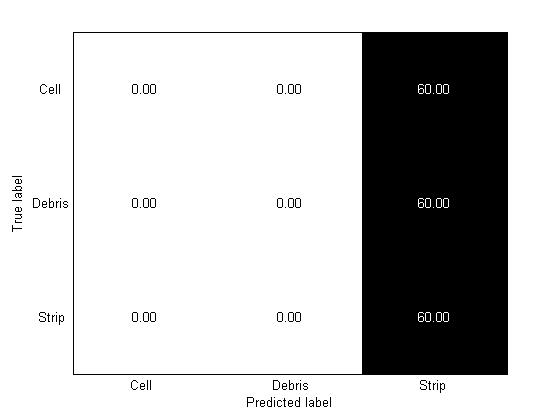
\includegraphics[width=\linewidth]{confusion_matrix/fig3_2}
\caption{A confusion matrix example when the classification accuracy is 33.33\% by using feature MIP}
\end{figure}
As it illustrates, all testing data are classified as strip type. In the meantime, the probabilities of the three classes are 0 for each testing example. In the previous section, we mentioned that the mechanism of multiple class classification is applying the one-vs-all method and selecting the maximum probability of class as the predicted result. Thus, when the accuracy is 33.33\%, the achieved classifier doesn't work for classification. The classifier with accuracy of 33.33\% is achieved by using feature s-MIP and p-MIP. Thus, we eliminate these two features. As Table 3.3 shows, the classifier can achieve accuracy that is more than 50.00\% using feature p-ASM, p-COR, p-SEN, p-ENT, and p-MAP. Based on these five features, we examine the remaining texture features and select six significant results as shown in Table 3.4.   
\begin{table}[!h]
\begin{center}
\renewcommand{\arraystretch}{0.5}
\begin{tabular}{|| c | c c c ||}
\hline
 Feature Combination& p-ENT\&p-CON & p-ASM\&s-CLS & p-SEN\&p-CON \\
 \hline
 Accuracy & 57.78\% & 57.22\% & 57.22\% \\
 \hline
 Confusion Matrix & Figure 3.3(a) & Figure 3.3(b) & Figure 3.3(c) \\
 \hline
 \hline
 Feature Combination& p-ASM\&p-DIS & p-MAP\&p-CON & p-ASM\&p-CON \\
 \hline
 Accuracy & 57.22\% & 57.22\% & 56.67\% \\
 \hline
 Confusion Matrix & Figure 3.3(d) & Figure 3.3(e) & Figure 3.3(f) \\
 \hline
\end{tabular}
\end{center}
\caption{The accuracy of SVM classifier trained on data examples with two feature parameters}
\end{table}
Due to these results, we add one more feature to increase the accuracy level. By comparing Table 3.4 with Table 3.3, we discover that the feature parameter contributing low accuracy is able to improve the performance of the classifier using another feature contributing high accuracy. For example, when training the classifier on the data with feature parameter p-DIS, the accuracy is 26.67\%. However, by training the classifier on the data with the feature combination consisting of p-DIS and p-ASM, the accuracy is 57.22\% which is higher than the accuracy of the classifier trained on data containing only the feature parameter p-ASM. 
\begin{figure}[!h]
\centering
  \begin{subfigure}[b]{0.3\textwidth}
    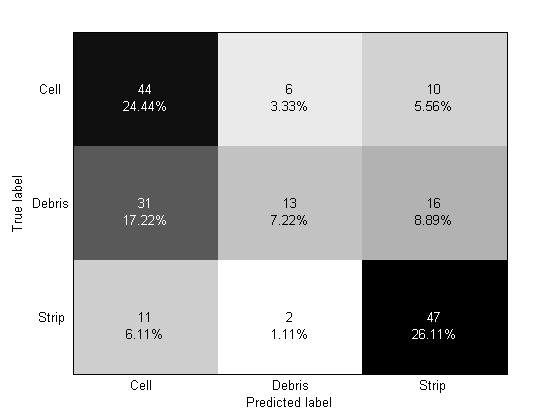
\includegraphics[width=\textwidth]{confusion_matrix/fig3_3a.jpg}
    \caption{}
  \end{subfigure}
  \begin{subfigure}[b]{0.3\textwidth}
    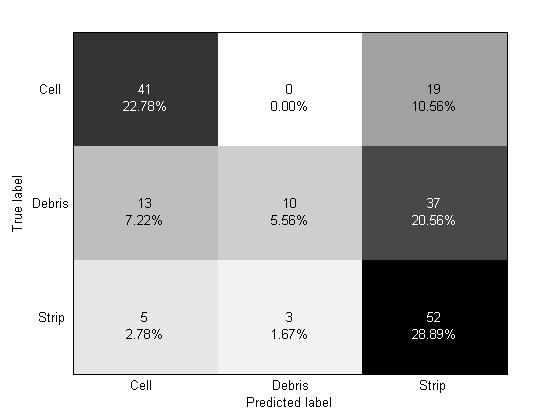
\includegraphics[width=\textwidth]{confusion_matrix/fig3_3b.jpg}
    \caption{}
  \end{subfigure}
  \begin{subfigure}[b]{0.3\textwidth}
    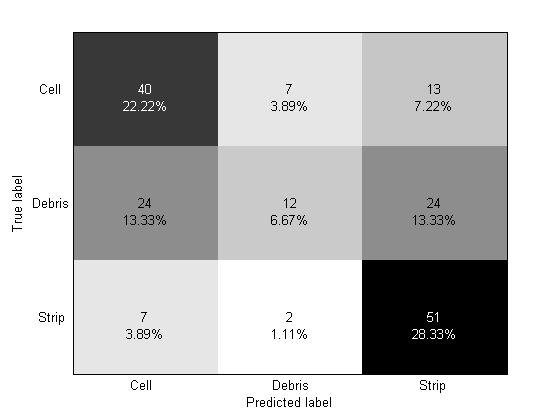
\includegraphics[width=\textwidth]{confusion_matrix/fig3_3c.jpg}
    \caption{}
  \end{subfigure}
  \begin{subfigure}[b]{0.3\textwidth}
    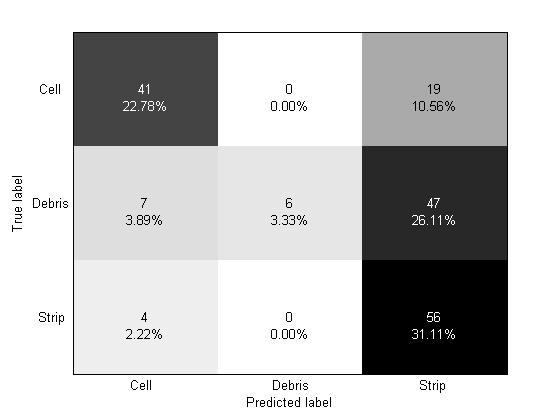
\includegraphics[width=\textwidth]{confusion_matrix/fig3_3d.jpg}
    \caption{}
  \end{subfigure}
  \begin{subfigure}[b]{0.3\textwidth}
    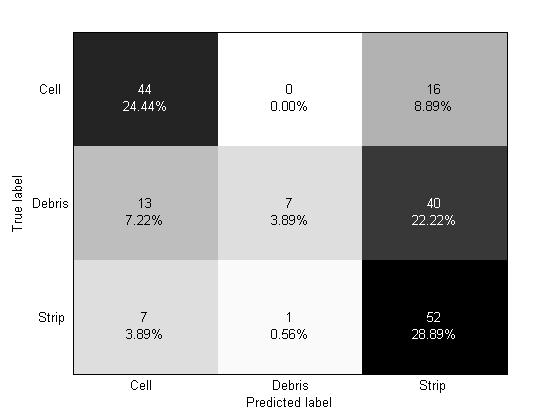
\includegraphics[width=\textwidth]{confusion_matrix/fig3_3e.jpg}
    \caption{}
  \end{subfigure}
  \begin{subfigure}[b]{0.3\textwidth}
    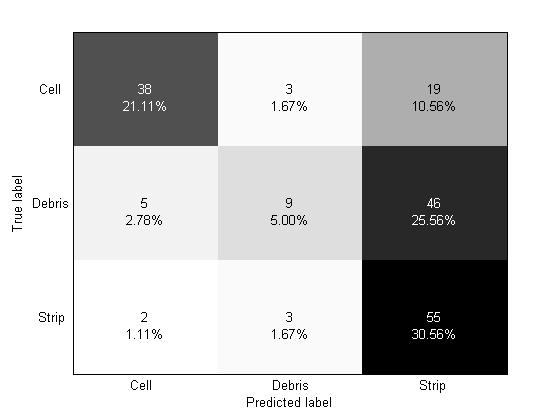
\includegraphics[width=\textwidth]{confusion_matrix/fig3_3f.jpg}
    \caption{}
  \end{subfigure}
  \caption{Confusion matrix of the SVM classifier trained on data with two feature parameters}
\end{figure}
Based on the result in Table 3.4, we achieve the accuracy of the SVM classifier trained on the data with three feature parameters shown in Table 3.5. All the combinations as Table 3.5 shown are evolved from the significant four combinations shown in Table 3.4 by adding new feature parameters selected from the remaining feature parameters. 
\begin{table}[!h]
\begin{center}
\renewcommand{\arraystretch}{0.5}
\begin{tabular}{|| c | c c ||}
\hline
 Feature Combination & p-ENT\;p-CON\&s-CLS & p-ENT\;p-CON\&s-CLP  \\
 \hline
 Accuracy & 60.56\% & 60.00\% \\
 \hline
 Confusion Matrix & Figure 3.4(a) & Figure 3.4(b)  \\
 \hline
 \hline
 Feature Combination & p-ASM\;p-CON\&s-CLP & p-SEN\;p-CON\&s-CLP \\
 \hline
 Accuracy & 59.44\% & 60.56\% \\
 \hline
 Confusion Matrix & Figure 3.4(c) & Figure 3.4(d)  \\
 \hline
 \hline
  Feature Combination & p-MAP\;p-CON\&s-VAR & p-MAP\;p-CON\&s-SEN \\
 \hline
 Accuracy & 60.00\% & 60.56\% \\
 \hline
 Confusion Matrix & Figure 3.4(e) & Figure 3.4(f)  \\
 \hline
\end{tabular}
\end{center}
\caption{The accuracy of SVM classifier trained on 360 data examples with three feature parameters}
\end{table}
\begin{figure}[!h]
\centering
  \begin{subfigure}[b]{0.3\textwidth}
    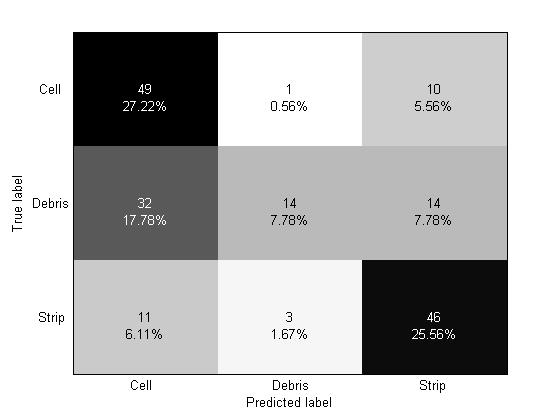
\includegraphics[width=\textwidth]{confusion_matrix/fig3_4a.jpg}
    \caption{}
  \end{subfigure}
  \begin{subfigure}[b]{0.3\textwidth}
    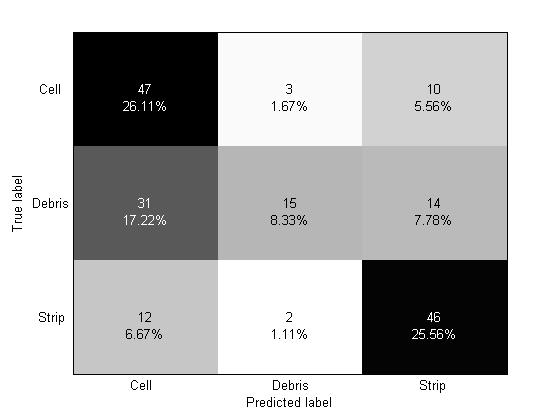
\includegraphics[width=\textwidth]{confusion_matrix/fig3_4b.jpg}
    \caption{}
  \end{subfigure}
  \begin{subfigure}[b]{0.3\textwidth}
    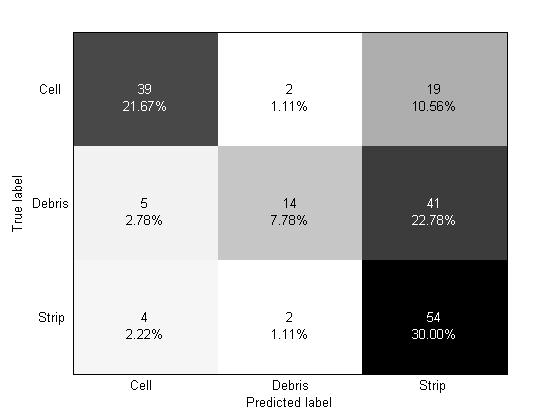
\includegraphics[width=\textwidth]{confusion_matrix/fig3_4c.jpg}
    \caption{}
  \end{subfigure}
  \begin{subfigure}[b]{0.3\textwidth}
    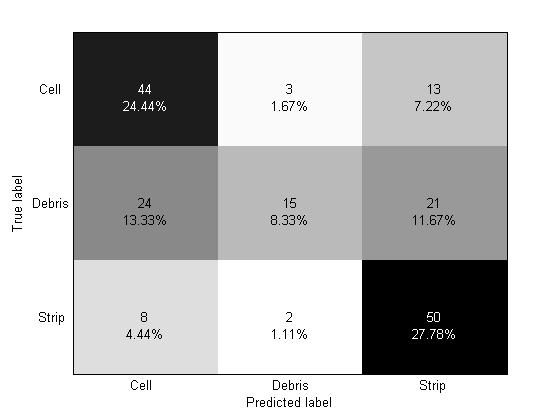
\includegraphics[width=\textwidth]{confusion_matrix/fig3_4d.jpg}
    \caption{}
  \end{subfigure}
  \begin{subfigure}[b]{0.3\textwidth}
    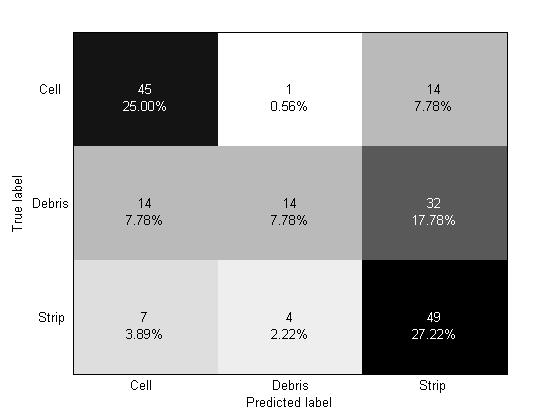
\includegraphics[width=\textwidth]{confusion_matrix/fig3_4e.jpg}
    \caption{}
  \end{subfigure}
  \begin{subfigure}[b]{0.3\textwidth}
    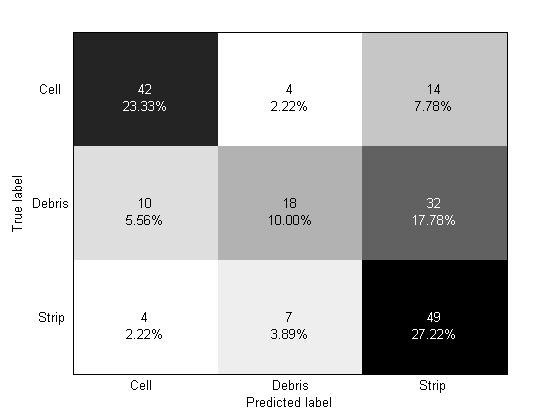
\includegraphics[width=\textwidth]{confusion_matrix/fig3_4f.jpg}
    \caption{}
  \end{subfigure}
  \caption{Confusion matrix of the SVM classifier trained on data examples with three feature parameters}
\end{figure}
The confusion matrix presents the visualization of a classifier's performance. We can see from Figure 3.3 that the classifier has trouble in distinguishing between the type cell and debris using feature p-ENT and p-CON and between the type debris and strip using the rest combinations in Table 3.4. After comparing the confusion matrix in Figures 3.3 and 3.4, adding new feature parameters mitigates the trouble.   
\begin{table}[!h]
\begin{center}
\renewcommand{\arraystretch}{0.7}
\begin{tabular}{|| c | c ||}
\hline
 Feature Combination & Accuracy  \\
\hline
 p-ENT\;p-CON\;s-CLS\&s-COR & 61.11\% \\
 p-ENT\;p-CON\;s-CLP\&s-COR & 61.11\% \\
 p-SEN\;p-CON\;s-CLP\&p-SAV & 61.67\% \\
 p-SEN\;p-CON\;s-CLP\&p-MEA & 61.67\% \\
 p-MAP\;p-CON\;s-VAR\&p-SAV & 61.67\% \\
 p-MAP\;p-CON\;s-VAR\&p-MEA & 61.67\% \\
\hline
\end{tabular}
\end{center}
\caption{The accuracy of SVM classifier trained on 360 data examples with four feature parameters}
\end{table}
Table 3.6 indicates that the highest accuracy level increases from 60.56\% to 61.67\% by adding a new feature. For example, the texture feature p-SVA is added into the combination including s-CLP, p-CON and p-SEN. In addition, we can find a situation in which adding either s-CLS or s-CLP can result in the same level of accuracy as well as adding either p-SAV or p-MEA. We introduce the line chart of these four texture features as Figure 3.5 shows. 
\begin{figure}[!h]
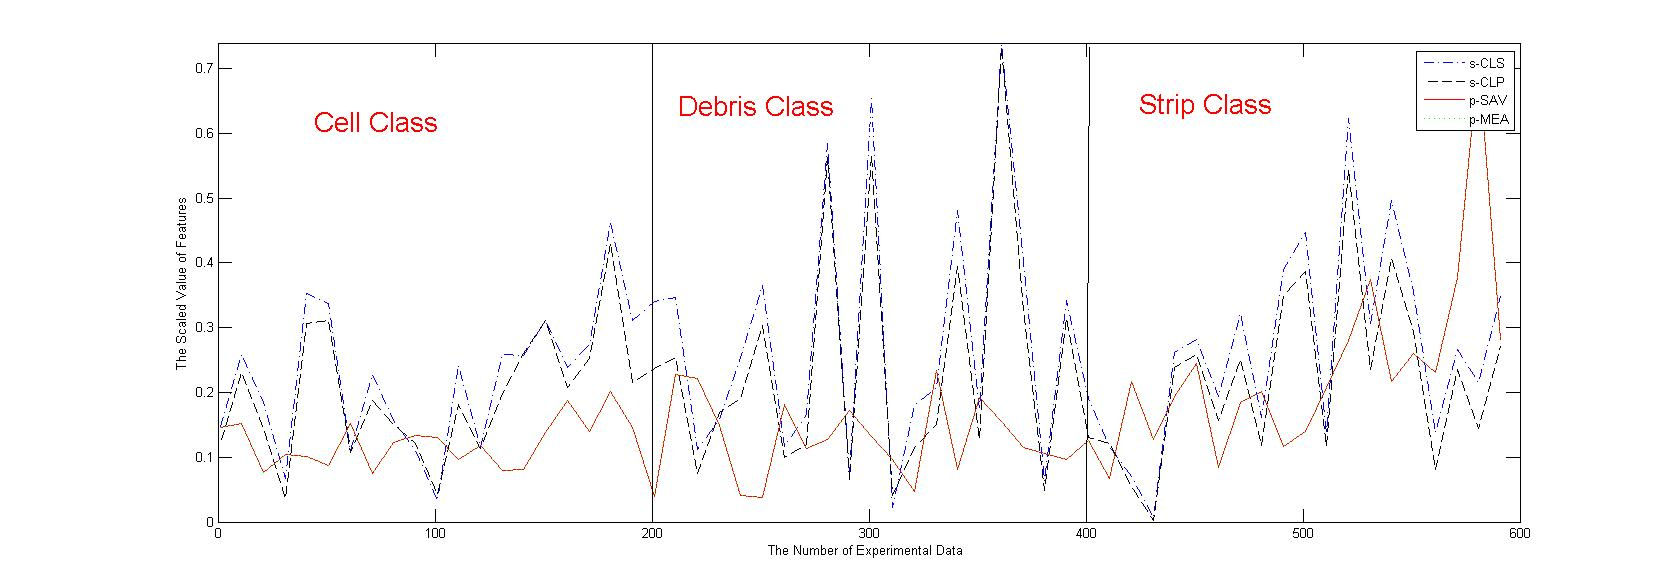
\includegraphics[width=\linewidth]{fig3_5}
\caption{The line chart for four texture features}
\end{figure}
In the figure, we can obviously see the correlation between two texture features. Especially, the feature p-SAV and p-MEA have the same values after scaling. Thus, adding feature p-SAV or p-MEA makes no difference in increasing the accuracy of the classifier. However, adding the feature s-CLS and the feature s-CLP may produce different results. Table 3.7 shows the accuracy of experimental data with five feature parameters. 
\begin{table}[!h]
\begin{center}
\renewcommand{\arraystretch}{0.7}
\begin{tabular}{|| c | c ||}
\hline
 Feature Combination & Accuracy  \\
\hline
 p-ENT\;p-CON\;s-CLS\;s-COR\&p-DIS & 62.22\% \\
 p-ENT\;p-CON\;s-CLP\;s-COR\&p-DIS & 59.44\% \\
 p-SEN\;p-CON\;s-CLP\;p-SAV\&s-COR & 61.67\% \\
 p-SEN\;p-CON\;s-CLP\;p-MEA\&s-COR & 61.67\% \\
 p-MAP\;p-CON\;s-VAR\;p-SAV\&p-SVA & 62.78\% \\
\hline
\end{tabular}
\end{center}
\caption{The accuracy of SVM classifier trained on 360 data examples with five feature parameters}
\end{table}
As Table 3.7 presents, by adding feature p-DIS, the combination with feature s-CLS results in increased accuracy, while the combination with feature s-CLP results in decreased accuracy. This result indicates that although feature s-CLS and s-CLP are correlated, they can be affected by another feature. By contrast, the third row and fourth row results denote that feature p-SAV and p-MEA are not affected by adding new features because they are considered as one feature after scaling. Currently, the highest accuracy of the SVM classifier trained on the data with the feature combination including p-MAP, p-CON, s-VAR, p-SAV and p-SVA is 62.78\%. When adding one more feature into this combination, the accuracy decreases to 62.22\%. Nevertheless, the combination including p-ENT, p-CON, s-CLS, s-COR and p-DIS results in higher accuracy by adding feature p-SEN as Table 3.8 shows.
\begin{table}[!h]
\begin{center}
\renewcommand{\arraystretch}{0.7}
\begin{tabular}{|| c | c ||}
\hline
 Feature Combination & Accuracy  \\
\hline
 Six Features &\\
\hline
 p-ENT\;p-CON\;s-CLS\;s-COR\;p-DIS\&p-SEN & 63.33\% \\
 p-MAP\;p-CON\;s-VAR\;p-SAV\;p-SVA\&p-DIS & 62.22\% \\
\hline
 Seven Features & \\
\hline
 p-ENT\;p-CON\;s-CLS\;s-COR\;p-DIS\;p-SEN\&p-VAR & 63.89\% \\
 \hline
 Eight Features & \\
\hline
 p-ENT\;p-CON\;s-CLS\;s-COR\;p-DIS\;p-SEN\;p-VAR\&p-CLP & 63.89\% \\
  \hline
 Nine Features & \\
\hline
 p-ENT\;p-CON\;s-CLS\;s-COR\;p-DIS\;p-SEN\;p-VAR\;p-CLP\&p-SVA & 62.78\% \\
\hline
\end{tabular}
\end{center}
\caption{The accuracy of SVM classifier trained on 360 data examples with more than five feature parameters}
\end{table}
After continuing adding feature p-VAR, the accuracy of the SVM classifier reaches the peak because adding more features cannot result in increased accuracy. Instead, when adding the feature p-SVA, the accuracy begins to decrease as Table 3.8 shows. In the meantime, a line chart in Figure 3.6 summarizes the results obtained in each step. 
\begin{figure}[!h]
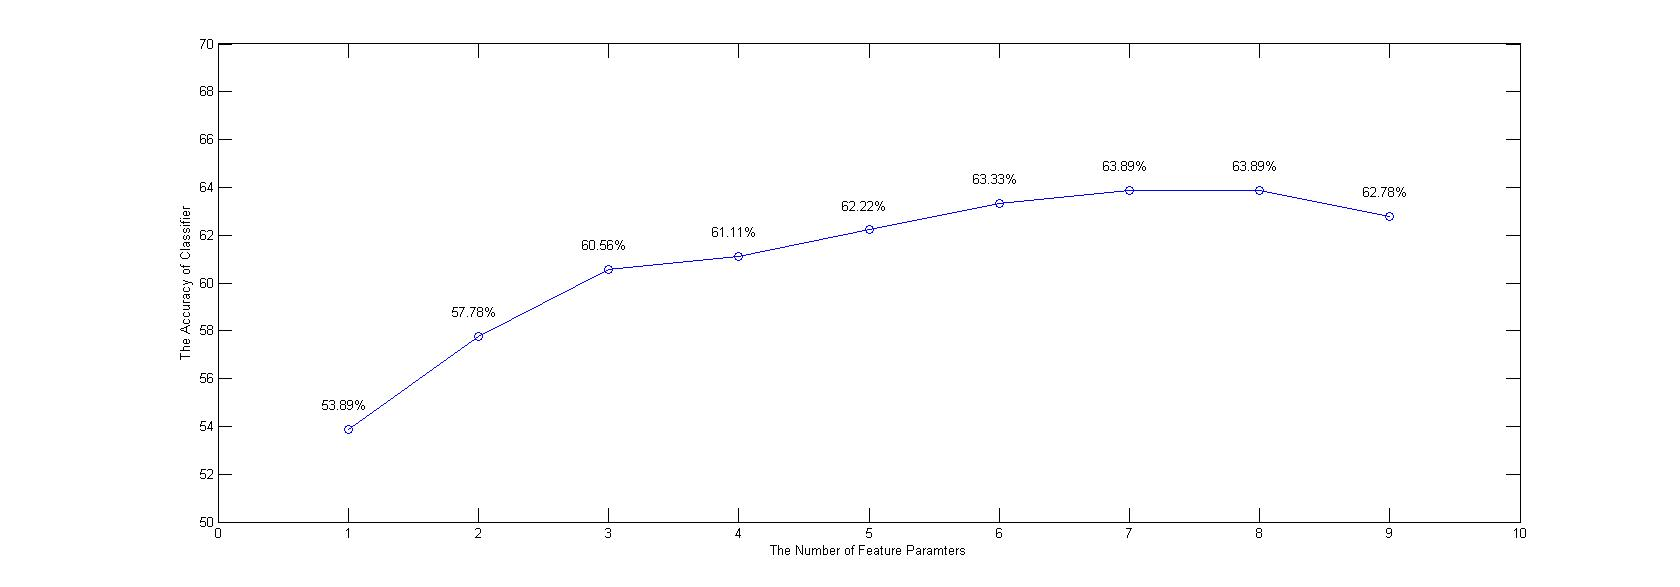
\includegraphics[width=\linewidth]{fig3_6}
\caption{One scenario of selecting feature parameters using the adding features approach (600 experimental data)}
\end{figure}
Therefore, we get the highest accuracy of 63.89\% by using the feature combination consisting of s-COR, s-CLS, p-CON, p-ENT, p-DIS, p-SEN and p-VAR. By applying this approach, we select eight texture features, and achieve the suitable SVM classifier with the highest accuracy by using these selected feature parameters.\par
In real situations, even though we achieve the classifier with the highest accuracy, it sometimes can't generalize to new examples. This is called classifier overfitting which describes the situation when the the classifier fits the training set very well. In other words, the SVM classifier is overly optimistic. Thus, validating the classifier is necessary. We extracted 20 data examples from each class, and a validating data set was constructed with total 60 data examples. By adding these data examples into training data set, the accuracy of the classifier decreases from 63.89\% to 41.11\%. The result reveals the fact that the previous classifier is overfitted with the specific feature parameter combination. To further examine the situation, we apply a common method called k-folder cross-validation in the training data set. Through specifying the parameter k with the value 5, we achieve the result for each folder as Table 3.9 shows.  
\begin{table}[!h]
\begin{center}
\begin{tabular}{||c c | c c ||}
\hline
Subset Index & Accuracy & Subset Index & Accuracy \\[0.7ex]
\hline\hline
1 & 43.06\% & 4 & 44.44\% \\
2 & 47.22\% & 5 & 51.39\% \\
3 & 45.83\% &  &  \\
\hline
 & & Average & 46.39\% \\
\hline
\end{tabular}
\caption {five-folder cross-validation result of SVM classifier}
\end{center}
\end{table}
From the table, we can see the average accuracy level is 46.39\% which is far below the highest accuracy level 63.89\%. As a result, the validation process confirms the fact that the SVM classifier achieved in the previous experiment is neither stable nor general. \par
The previous experiment and classifier validation process reveal the problem that the SVM classifier with an accuracy level of 63.89\% fits the training data set too well to generalize to new examples. Once new examples are added, the classifier cannot maintain its accuracy anymore. To solve this problem, we involved more training data to improve the generalization of the classifier. At this time, we applied all 3000 experimental data. Within the 3000 data, there are 957 data samples labeled as Cell, 1555 data samples labeled as Debris and 488 data samples labeled as Strip. To construct the training data set, we selected 1200 out of 3000 experimental data samples. Also, we selected 600 out of 3000 data samples as the testing data set and the rest as the validating data set. Then, by repeating the experiment with the new experimental data, we achieved the each level of accuracy of the SVM classifier trained on the data with a single feature as Table 3.10 shows. 
\begin{table}[!h]
\begin{center}
\renewcommand{\arraystretch}{0.5}
\begin{tabular}{||c c c c c c ||}
\hline
Index & Feature & Accuracy & Index & Feature & Accuracy \\[0.7ex]
\hline\hline
1 & s-ASM & 53.33\% & 21 & p-ASM & 56.50\% \\
2 & s-CON & 53.33\% & 22 & p-CON & 53.33\% \\
3 & s-COR & 53.33\% & 23 & p-COR & 53.33\% \\
4 & s-VAR & 53.33\% & 24 & p-VAR & 53.33\% \\
5 & s-IDM & 53.33\% & 25 & p-IDM & 53.33\% \\
6 & s-SAV & 53.33\% & 26 & p-SAV & 53.33\% \\
7 & s-SEN & 53.33\% & 27 & p-SEN & 53.33\% \\
8 & s-SVA & 53.33\% & 28 & p-SVA & 53.33\% \\
9 & s-ENT & 53.33\% & 29 & p-ENT & 55.67\% \\
10 & s-DEN & 53.33\% & 30 & p-DEN & 53.33\% \\
11 & s-DVA & 53.33\% & 31 & p-DVA & 53.33\% \\
12 & s-DIS & 53.33\% & 32 & p-DIS & 53.33\% \\
13 & s-CLS & 53.33\% & 33 & p-CLS & 53.33\% \\
14 & s-CLP & 53.33\% & 34 & p-CLP & 53.33\% \\
16 & s-MAP & 53.33\% & 36 & p-MAP & 55.50\% \\
17 & s-MEA & 53.33\% & 37 & p-MEA & 53.33\% \\
\hline
\end{tabular}
\caption {The accuracy of the SVM classifier trained on 1200 experimental data examples with single feature parameter}
\end{center}
\end{table}
In the Table 3.10 we can see that only using feature p-ASM, p-ENT, and p-MAP for classification can achieve a level of accuracy that is more than 53.33\%. Since there are 320 debris data samples in the testing data set, the accuracy of 53.33\% has the same meaning as the accuracy of 33.33\%. Based on the three features, we select one more feature to evolve the combination with two feature parameters and list six results with high accuracy in Table 3.11.
\begin{table}[!h]
\begin{center}
\renewcommand{\arraystretch}{0.5}
\begin{tabular}{|| c | c c c ||}
\hline
 Feature Combination& p-CON\&p-MAP & p-ASM\&p-CON & p-ENT\&p-DIS \\
 \hline
 Accuracy & 58.33\% & 58.00\% & 58.00\% \\
 \hline
 \hline
 Feature Combination& p-CON\&p-ENT & s-SAV\&p-ASM & p-ASM\&p-SAV \\
 \hline
 Accuracy & 57.83\% & 57.17\% & 57.17\% \\
 \hline
\end{tabular}
\end{center}
\caption{The accuracy of SVM classifier trained on 1200 data examples with two feature parameters}
\end{table}
The result in Table 3.11 indicates that the accuracy increases by adding another feature parameter. In general, each feature parameter in the same combination is from a different group. For instance, the feature p-CON comes from group 1 which is the measures of Contrast, while the feature p-MAP comes from group 2 which is the measures of Uniformity or Orderliness of pixels. For each combination in Table 3.11, we add one more feature parameter and achieve higher accuracy as shown in Table 3.12. 
\begin{table}[!h]
\begin{center}
\renewcommand{\arraystretch}{0.5}
\begin{tabular}{|| c | c c ||}
\hline
 Feature Combination & p-CON\;p-MAP\&p-COR & p-ASM\;p-CON\&p-SEN  \\
 \hline
 Accuracy & 59.67\% & 58.50\% \\
 \hline
 \hline
 Feature Combination & p-ENT\;p-DIS\&s-SAV & p-CON\;p-ENT\&s-SAV \\
 \hline
 Accuracy & 59.33\% & 59.67\% \\
 \hline
 \hline
  Feature Combination & s-SAV\;p-ASM\&p-CON & p-ASM\;p-SAV\&p-CON \\
 \hline
 Accuracy & 58.00\% & 57.83\% \\
 \hline
\end{tabular}
\end{center}
\caption{The accuracy of SVM classifier trained on 1200 data examples with three feature parameters}
\end{table}
For most combinations containing three feature parameters, each feature comes from a different group as we mentioned for the combination with two feature parameters. By adding one more feature into the combination, we achieved the result shown in Table 3.13. 
\begin{table}[!h]
\begin{center}
\renewcommand{\arraystretch}{0.7}
\begin{tabular}{|| c | c ||}
\hline
 Feature Combination & Accuracy  \\
\hline
 p-CON\;p-MAP\;p-COR\&s-MAP & 60.17\% \\
 p-ASM\;p-CON\;p-SEN\&s-ASM & 58.83\% \\
 p-ENT\;p-DIS\;s-SAV\&s-MEA & 59.67\% \\
 p-CON\;p-ENT\;s-SAV\&s-MEA & 60.67\% \\
 s-SAV\;p-ASM\;p-CON\&p-ENT & 59.17\% \\
 p-ASM\;p-SAV\;p-CON\&p-SEN & 58.67\% \\
\hline
\end{tabular}
\end{center}
\caption{The accuracy of SVM classifier trained on 1200 data examples with four feature parameters}
\end{table}
For each combination in Table 3.12, the accuracy increases through adding a new feature parameter. When the number of feature parameters is five, the accuracy is increasing as is shown in Table 3.14.
\begin{table}[!h]
\begin{center}
\renewcommand{\arraystretch}{0.7}
\begin{tabular}{|| c | c ||}
\hline
 Feature Combination & Accuracy  \\
\hline
 p-CON\;p-MAP\;p-COR\;s-MAP\&s-SEN & 60.33\% \\
 p-ASM\;p-CON\;p-SEN\;s-ASM\&s-SAV & 59.67\% \\
 p-ENT\;p-DIS\;s-SAV\;s-MEA\&s-ASM & 60.67\% \\
 p-CON\;p-ENT\;s-SAV\;s-MEA\&s-MAP & 60.83\% \\
 s-SAV\;p-ASM\;p-CON\;p-ENT\&s-IDM & 59.83\% \\
 p-ASM\;p-SAV\;p-CON\;p-SEN\&s-VAR & 59.17\% \\
\hline
\end{tabular}
\end{center}
\caption{The accuracy of SVM classifier trained on 1200 data examples with five feature parameters}
\end{table}
However, when the number of feature parameters reaches six, the SVM classifier cannot be improved by using some feature parameter combinations. For example, the SVM classifier with accuracy of 59.67\% no longer increases its accuracy when adding feature s-SAV. Furthermore, when adding feature s-SVA, the accuracy decreases. Considering this situation, we eliminate the classifiers with accuracy below 60\%.   
\begin{table}[!b]
\begin{center}
\renewcommand{\arraystretch}{0.7}
\begin{tabular}{|| c | c ||}
\hline
 Feature Combination & Accuracy  \\
\hline
 Six Features &\\
\hline
 p-CON\;p-MAP\;p-COR\;s-MAP\;s-SEN\&s-DIS & 60.67\% \\
 p-ENT\;p-DIS\;s-SAV\;s-MEA\;s-ASM\&s-MAP & 61.17\% \\
 p-CON\;p-ENT\;s-SAV\;s-MEA\;s-MAP\&p-SVA & 61.33\% \\
\hline
 Seven Features & \\
\hline
 p-CON\;p-MAP\;p-COR\;s-MAP\;s-SEN\;s-DIS\&s-CON & 60.67\% \\
 p-ENT\;p-DIS\;s-SAV\;s-MEA\;s-ASM\:s-MAP\&s-IDM & 61.50\% \\
 p-CON\;p-ENT\;s-SAV\;s-MEA\;s-MAP\;p-SVA\&s-CON & 61.33\% \\
 \hline
 Eight Features & \\
\hline
 p-CON\;p-MAP\;p-COR\;s-MAP\;s-SEN\;s-DIS\;s-CON\&p-SAV & 60.83\% \\
 p-ENT\;p-DIS\;s-SAV\;s-MEA\;s-ASM\:s-MAP\;s-IDM\&p-CLS & 61.50\% \\
 p-CON\;p-ENT\;s-SAV\;s-MEA\;s-MAP\;p-SVA\;s-CON\&s-SEN & 61.33\% \\
\hline
 Nine Features & \\
\hline
  p-ENT\;p-DIS\;s-SAV\;s-MEA\;s-ASM &\\
  s-MAP\;s-IDM\;p-CLS\&s-DVA & 61.50\% \\
\hline
 Eleven Features & \\
\hline
 p-ENT\;p-DIS\;s-SAV\;s-MEA\;s-ASM &\\
 s-MAP\;s-IDM\;p-CLS\;s-DVA\;s-COR\&p-CLP & 61.67\% \\
\hline
 Twelve Features & \\
\hline
 p-ENT\;p-DIS\;s-SAV\;s-MEA\;s-ASM\;s-MAP &\\
 s-IDM\;p-CLS\;s-DVA\;s-COR\;p-CLP\&s-CLP & 61.33\% \\
\hline
\end{tabular}
\end{center}
\caption{The accuracy of SVM classifier trained on 1200 data examples with more than five feature parameters}
\end{table}
Thus, we have three SVM models left. With the number of feature parameters increased, the results of two classifiers reveal the fact that the accuracy can't grow. If we add two more feature parameters, the accuracy is still the same. Therefore, there is only one feature parameter combination remaining. Eventually, the SVM classifier reaches the highest accuracy of 61.67\% when it is trained on the data with 11 feature parameters which are s-ASM, s-COR, s-IDM, s-SAV, s-DVA, s-MAP, s-MEA, p-ENT, p-DIS, p-CLS and p-CLP. By adding the validating data set into the training data set, the accuracy of the selected model decreases 0.34\%. The slight change is acceptable since the experimental data we used are not ideal. Figure 3.7 presents a scenario in which the accuracy variation of  the SVM classifier with the number of feature parameters increases for this combination.
\begin{figure}
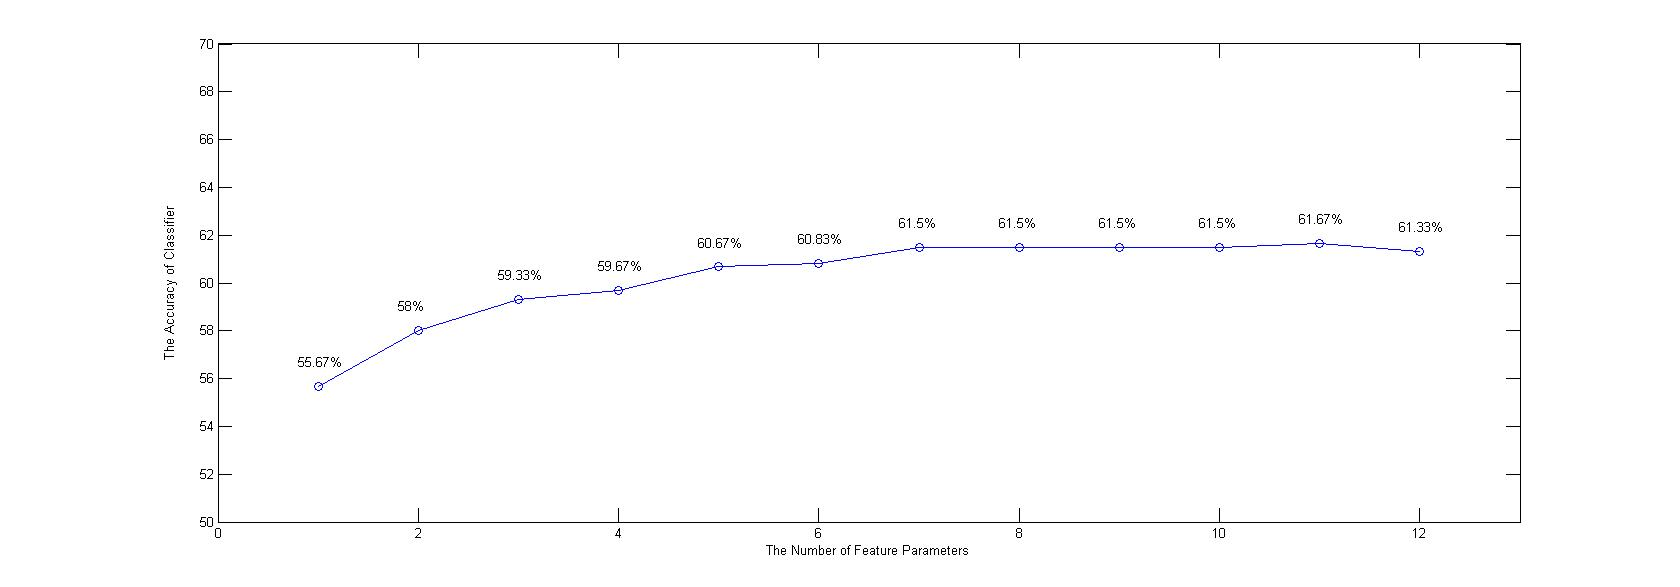
\includegraphics[width=\linewidth]{fig3_7}
\caption{One scenario of selecting feature parameters using adding feature approach (3000 experimental data)}
\end{figure}
The primary goal of selecting feature parameters is to prevent invalid texture features from affecting the accuracy of classification. Thus, the classifier trained on the data with all feature parameters would have lower accuracy than the one selected from the previous experiment. Through this approach, we achieve that the highest accuracy of the SVM classifier is 61.67\% by using 11 feature parameters. However, when training the SVM classifier with all 32 feature parameters, we attain a higher accuracy 64.17\%. Obviously, the previous experimental approach fails to reach the goal. To improve, another feature selection approach is proposed. In contrast to adding a feature parameter, we monitor the change of the SVM classifier's accuracy by directly removing the invalid feature parameter from the original combination containing all 32 feature parameters. First, we monitor the variations of accuracy level when removing a feature parameter. The accuracy is increased when the feature s-CON, p-ASM, p-ENT or p-MAP is removed from the combination shown in Table 3.16. 
\begin{table}[!h]
\begin{center}
\renewcommand{\arraystretch}{0.5}
\begin{tabular}{|| c | c | c c c||}
\hline
 Feature Removed & NONE & s-CON & p-ASM & p-MAP  \\
 \hline
 Accuracy & 64.17\% & 64.67\% & 65.00\% & 65.17\% \\
 \hline
\end{tabular}
\end{center}
\caption{The accuracy change of SVM classifier after removing a feature parameter from experimental data}
\end{table}
By comparing with Table 3.10, we achieve a totally conflicting result. For the previous experimental approach, a new feature parameter combination was always created due to the old combination with high accuracy of SVM classifier. Thus, the feature p-ASM, p-ENT and p-MAP are considered as the first feature parameters that are selected. However, the current experimental approach proves that these three feature parameters are invalid features and they may result in the lower accuracy of a classifier. After removing the feature p-MAP, we repeat the same process. The accuracy of the SVM classifier increases to 65.33\% by removing s-CON, s-SEN or s-MAP as shown in Table 3.17.
\begin{table}[!h]
\begin{center}
\renewcommand{\arraystretch}{0.5}
\begin{tabular}{|| c | c | c c ||}
\hline
 Feature Removed & p-MAP & p-MAP\&s-CON & p-MAP\&p-SVA \\
 \hline
 Accuracy & 65.17\% & 65.33\% & 65.33\% \\
 \hline
\end{tabular}
\end{center}
\caption{The accuracy change of SVM classifier after removing two feature parameters from experimental data}
\end{table}
Since the SVM classifier can reach the same level of accuracy by removing the feature s-CON or p-SVA, we examine separately for each feature parameter. Due to the combination removing the feature s-CON, the accuracy of the classifier increases to 65.50\% after the feature parameter s-COR, p-VAR or p-CLS is removed shown in Table 3.18. 
\begin{table}[!h]
\begin{center}
\renewcommand{\arraystretch}{0.5}
\begin{tabular}{|| c | c | c c c||}
\hline
 & Features Have Removed & & Feature Is Removed &\\
\hline
 Feature & p-MAP\&s-CON & s-COR & p-VAR & p-CLS\\
 \hline
 Accuracy & 65.33\% & 65.50\% & 65.50\% & 65.50\% \\
 \hline
 Feature & p-MAP\&p-SVA & & s-CON &\\
 \hline
 Accuracy & 65.33\% & & 65.17\% & \\
 \hline
\end{tabular}
\end{center}
\caption{The accuracy change of SVM classifier after removing three feature parameters from experimental data}
\end{table}
In addition, Table 3.18 presents another result that after removing feature p-SVA, the accuracy commences decreasing. Therefore, we start the first scenario from removing the feature s-COR.    
\begin{table}[!h]
\begin{center}
\renewcommand{\arraystretch}{0.5}
\begin{tabular}{|| c | c | c | c | c | c ||}
\hline
 Step & Feature & Accuracy & Step & Feature & Accuracy \\
\hline
 0 & p-MAP\;\&\;s-CON & 65.33\% & & & \\
\hline
 1 & s-COR & 65.50\% & 6 & p-DEN & 65.33\% \\
 2 & p-SVA & 65.50\% & 7 & s-CLS & 65.33\% \\
 3 & p-ASM & 65.50\% & 8 & s-CLP & 65.50\% \\
 4 & s-ENT & 65.50\% & 9 & s-SVA & 65.50\% \\
 5 & p-CLP & 65.50\% & 10 & p-VAR & 65.17\% \\
\hline
\end{tabular}
\end{center}
\caption{The first scenario of selecting a SVM classifier starting with removing feature s-COR}
\end{table}
However, by sequentially removing feature p-SVA, p-ASM, s-ENT, p-CLP, the highest accuracy is still 65.50\%. When removing feature p-DEN, the accuracy decreases. Even though the accuracy is back to 65.50\% by keeping removing feature s-CLP, it decrease significantly by removing feature p-VAR. Thus, we are unable to reach a higher accuracy by following the first scenario of selecting feature parameters for classification. 
We follow the same procedure and start examining the second scenario of selecting feature parameters shown in Table 3.20.
\begin{table}[!h]
\begin{center}
\renewcommand{\arraystretch}{0.5}
\begin{tabular}{|| c | c | c | c | c | c ||}
\hline
 Step & Feature & Accuracy & Step & Feature & Accuracy \\
\hline
 0 & p-MAP\;\&\;s-CON & 65.33\% & & & \\
\hline
 1 & p-VAR & 65.33\% & 4 & s-CLP & 65.50\% \\
 2 & p-CLS & 65.67\% & 5 & p-CLP & 65.17\% \\
 3 & p-SVA & 65.50\% &  &  & \\
\hline
\end{tabular}
\end{center}
\caption{The second scenario of selecting a SVM classifier starting with removing feature p-VAR}
\end{table}
The second scenario is simply. The accuracy reaches the peak when sequentially removing p-VAR and p-CLS. It decreases when removing more feature parameters. The third scenario of selecting feature parameters starts with removing feature p-CLS shown in Table 3.21. 
\begin{table}[!h]
\begin{center}
\renewcommand{\arraystretch}{0.5}
\begin{tabular}{|| c | c | c | c | c | c ||}
\hline
 Step & Feature & Accuracy & Step & Feature & Accuracy \\
\hline
 0 & p-MAP\;\&\;s-CON & 65.33\% & & & \\
\hline
 1 & p-CLS & 65.50\% & 6 & s-CLS & 65.50\% \\
 2 & p-SVA & 65.67\% & 7 & p-ASM & 65.50\% \\
 3 & s-CLP & 65.67\% & 8 & s-ASM & 65.50\% \\
 4 & p-CLP & 65.50\% & 9 & s-SEN & 65.33\% \\
 5 & s-COR & 65.67\% & & &  \\
\hline
\end{tabular}
\end{center}
\caption{The third scenario of selecting a SVM classifier starting with removing feature p-CLS}
\end{table}
It is more complex than the second scenario. We can select three feature combinations from it. Figure 3.8 presents a line chart to visualize the accuracy variation of the third scenario.
\begin{figure}
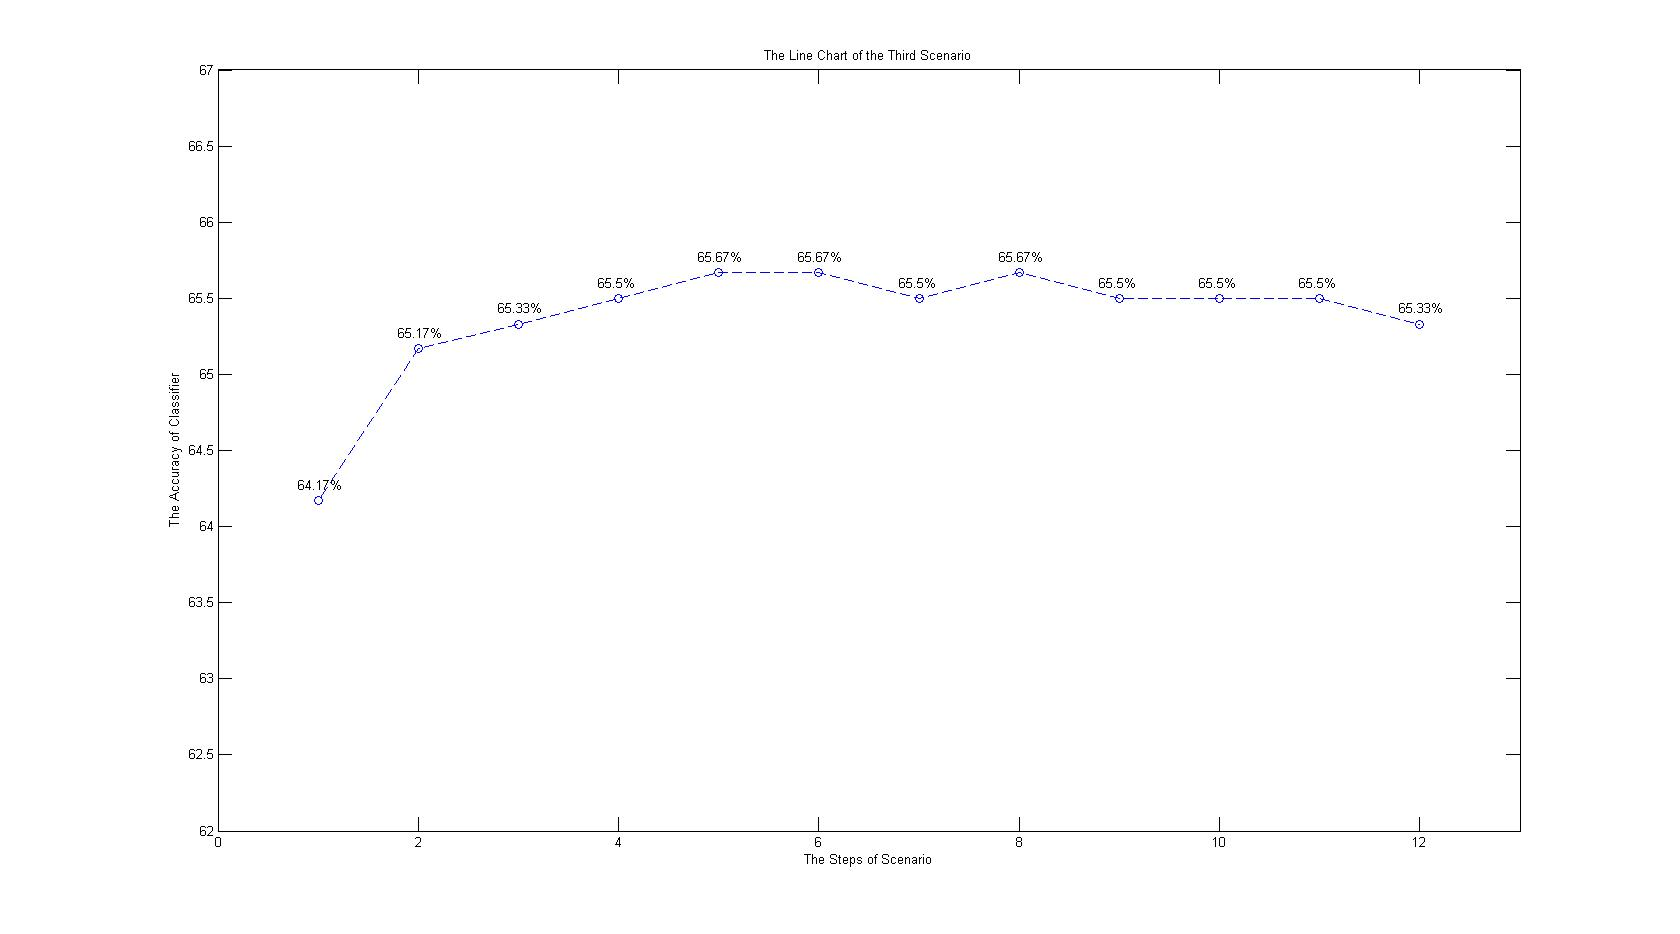
\includegraphics[width=\linewidth]{fig3_8c}
\caption{One scenario of selecting feature parameters using backward propagation approach}
\end{figure}
We create four SVM classifiers using the feature parameter combinations from second and third scenario shown in Table 3.22. 
\begin{table}[!h]
\begin{center}
\renewcommand{\arraystretch}{0.8}
\begin{tabular}{|| c | c | c | c | c ||}
\hline
 Classifier & Classifier & Number of & Accuracy & Accuracy \\
 Index & From Scenario &  Features & Before Validation & After Validation \\
\hline
 1 & 2 &28 & 65.67\% & 65.67\% \\
 2 & 3 &28 & 65.67\% & 65.50\% \\
 3 & 3 &27 & 65.67\% & 65.50\% \\
 4 & 3 &25 & 65.67\% & 65.50\% \\
\hline 
\end{tabular}
\end{center}
\caption{The comparison among four classifiers}
\end{table}
The table illustrates the basic information for the classifier using four selected feature combination for classification. The first classifier is created using the combination selected from the second scenario and the rest classifiers are created using the combinations from the third scenario. To select the best feature parameter combination, we perform the validation by adding validating data set in training data set for each classifier. As Table 3.22 shown, the classifier trained on data with feature combination selected from second scenario is the best. In addition, we apply the 10-folder cross-validation method in the first classifier. The result is shown in Table 3.23. 
\begin{table}[!h]
\begin{center}
\begin{tabular}{||c c | c c ||}
\hline
Subset Index & Accuracy & Subset Index & Accuracy \\[0.7ex]
\hline\hline
1 & 70.50\% & 6 & 70.50\% \\
2 & 65.50\% & 7 & 64.00\% \\
3 & 67.50\% & 8 & 60.00\% \\
4 & 65.50\% & 9 & 62.50\% \\
5 & 65.00\% & 10 & 67.00\%  \\
\hline
 & & Average & 65.80\% \\
\hline
\end{tabular}
\caption {10-folder cross-validation result of SVM classifier}
\end{center}
\end{table}
The average accuracy of the cross-validation further confirm the classifier we selected is satisfied with our expectation. 
\subsection{The Improvement of SVM Classifier}
In this research, we apply the RBF kernel which has two important parameters C and $\gamma$. Practically speaking, a SVM classifier can be further optimized by identifying the best parameter pair of (C, $\gamma$). We estimate the parameter pair of (C, $\gamma$) to C = $2^0$ and $\gamma = 0.07$ as the default values and achieve the SVM classifier with accuracy 65.67\%. Then, we try all combinations between parameter C from $2^{-5}$ to $2^{15}$ and $\gamma$ from $2^{-15}$ to $2^3$ (for example, C = $2^{-5}$, $2^{-4}$, $\ldots$, $2^{15}$, $\gamma$ = $2^{-15}$, $2^{-14}$, $\ldots$, $2^3$) to identify the best parameter pair. We list some of the results in Table 3.24. 
\begin{table}[!h]
\begin{center}
\renewcommand{\arraystretch}{0.8}
\begin{tabular}{||c| c c c c c c c c c ||}
\hline
 \backslashbox{C}{$\gamma$} & $2^{-15}$ & $2^{-14}$ & $\ldots$ & $2^{-3}$ & $2^{-2}$ & $2^{-1}$ & $\ldots$ & $2^2$ & $2^3$ \\
\hline
 $2^{-5}$ & 53.33 & 53.33 & $\ldots$ & 53.33 & 56.67 & 58.50 & $\ldots$ & 65.33 & 59.33 \\
 $2^{-4}$ & 53.33 & 53.33 & $\ldots$ & 57.00 & 58.67 & 62.17 & $\ldots$ 
& 69.00 & 68.67 \\
 $\ldots$ & $\ldots$ & $\ldots$ & $\ldots$ & $\ldots$ & $\ldots$ & $\ldots$ & $\ldots$ 
& $\ldots$ & $\ldots$ \\
 $2^{9}$ & 58.16 & 59.00 & $\ldots$ & 78.33 & 79.67 & \cellcolor{blue!25}80.00 & $\ldots$ 
& 66.00 & 67.67 \\
 $\ldots$ & $\ldots$ & $\ldots$ & $\ldots$ & $\ldots$ & $\ldots$ & $\ldots$ & $\ldots$ 
& $\ldots$ & $\ldots$ \\
 $2^{12}$ & 63.00 & 64.83 & $\ldots$ & \cellcolor{blue!25}80.33 & 79.50 & 75.50 & $\ldots$ 
& 65.83 & 67.67 \\
 $\ldots$ & $\ldots$ & $\ldots$ & $\ldots$ & $\ldots$ & $\ldots$ & $\ldots$ & $\ldots$ 
& $\ldots$ & $\ldots$ \\
 $2^{14}$ & 67.33 & 67.83 & $\ldots$ & 79.33 & 76.67 & 74.33 & $\ldots$ 
& 65.83 & 67.67 \\
 $2^{15}$ & 67.83 & 67.83 & $\ldots$ & 79.33 & 75.33 & 72.83 & $\ldots$ 
& 65.83 & 67.67 \\
\hline
\end{tabular}
\caption {The various pairs of (C, $\gamma$) values}
\end{center}
\end{table}
Based on the results, the accuracy of the SVM classifier is 80.33\% when C=$2^{12}$ and $\gamma = 2^{-3}$ and 80.00\% when C=$2^{9}$ and $\gamma = 2^{-1}$. The results after involving the validating data set are shown in Table 3.25. 
\begin{table}[!h]
\begin{center}
\renewcommand{\arraystretch}{0.8}
\begin{tabular}{|| c | c | c | c ||}
\hline
 Classifier Index & pair of (C, $\gamma$) & Accuracy & Accuracy \\
 & & Before Validation & After Validation \\
\hline
 1 & ($2^{9}$, $\gamma = 2^{-1}$) & 80.00\% & 78.83\% \\
 2 & ($2^{12}$, $\gamma = 2^{-3}$) & 80.33\% & 80.5\% \\
\hline 
\end{tabular}
\end{center}
\caption{The comparison between two pairs of (C, $\gamma$)}
\end{table}
The variation in accuracy of the first classifier is larger than the variation in accuracy of the second classifier. Therefore, we consider the first classifier as higher risk than the second one in failing to generalize to new examples. To conclude, we consider the second SVM classifier as the best experimental result and achieve the confusion matrix as Figure 3.9 shows. 
\begin{figure}[!b]
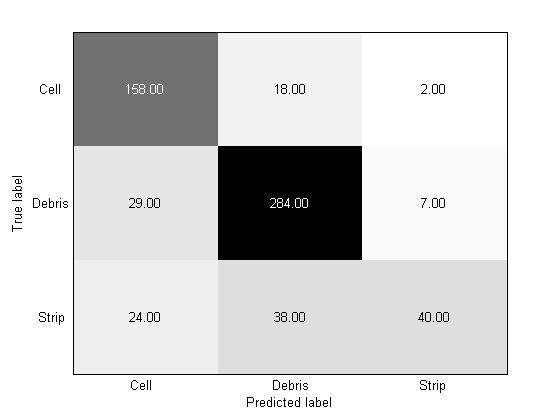
\includegraphics[width=\linewidth]{fig3_9}
\caption{The confusion matrix of the best SVM classifier}
\end{figure}
\subsection{Comparative Work}
In this experiment, we combine two diffraction images together to improve their representation. We select 28 feature parameters applied in SVM and achieve the classification accuracy of 80.33\% after assigning the parameter pair of ($2^{12}$, $2^{-3}$). We also apply the approach of extensive feature correlation study (EFCS) that Thati used in his research on feature selection\cite{Thati} for comparison. By selecting 200 examples from each type of diffraction image, we build three trends of various features for each feature group shown in Figures 3.10, 3.11 and 3.12. From the three figures, we can see the correlation among feature parameters. 
\begin{figure}
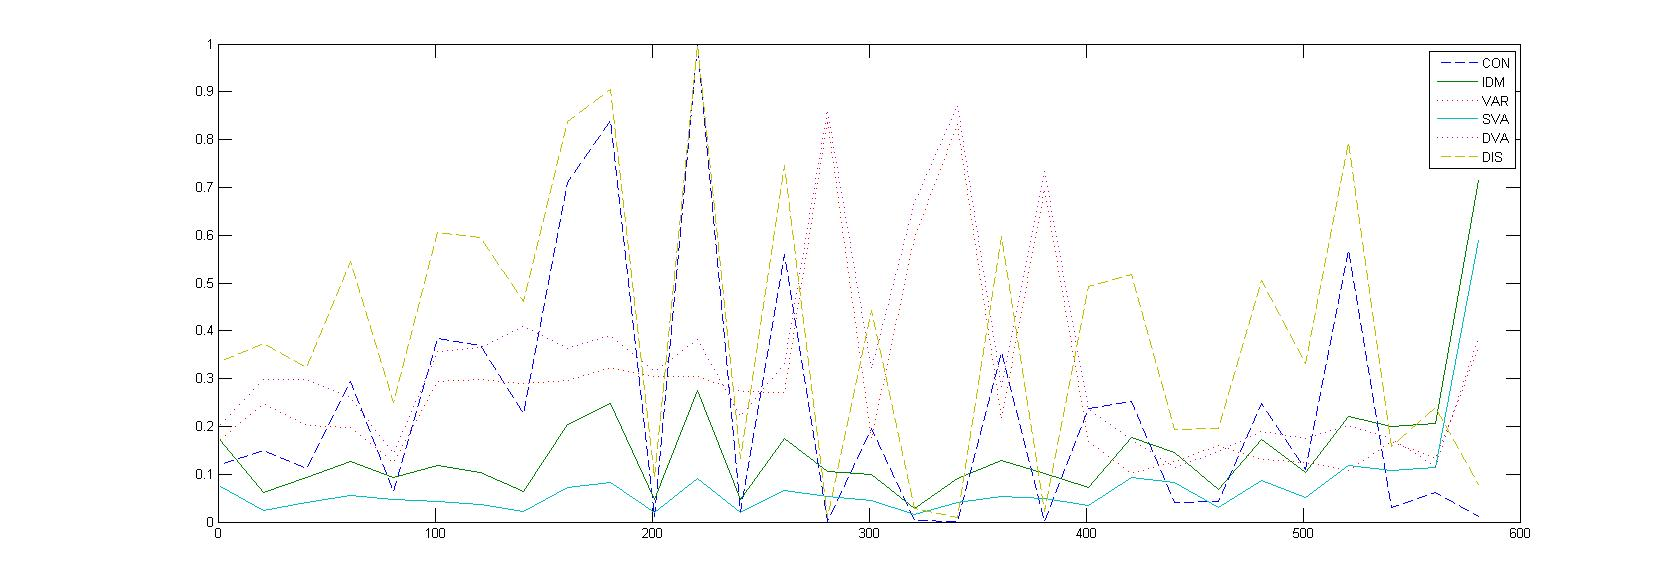
\includegraphics[width=\linewidth]{p_feature_group1}
\caption{The trends of various features in Group 1}
\end{figure}
\begin{figure}
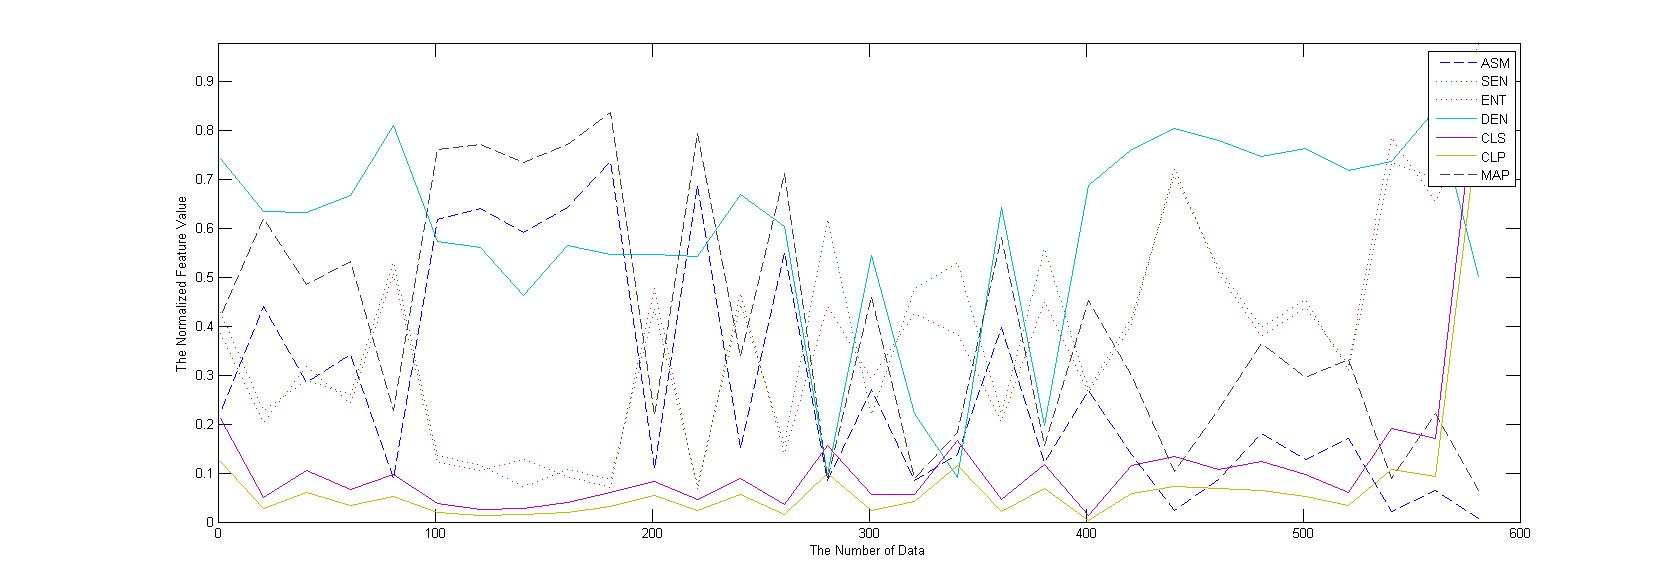
\includegraphics[width=\linewidth]{p_feature_group2}
\caption{The trends of various features in Group 2}
\end{figure}
\begin{figure}[!t]
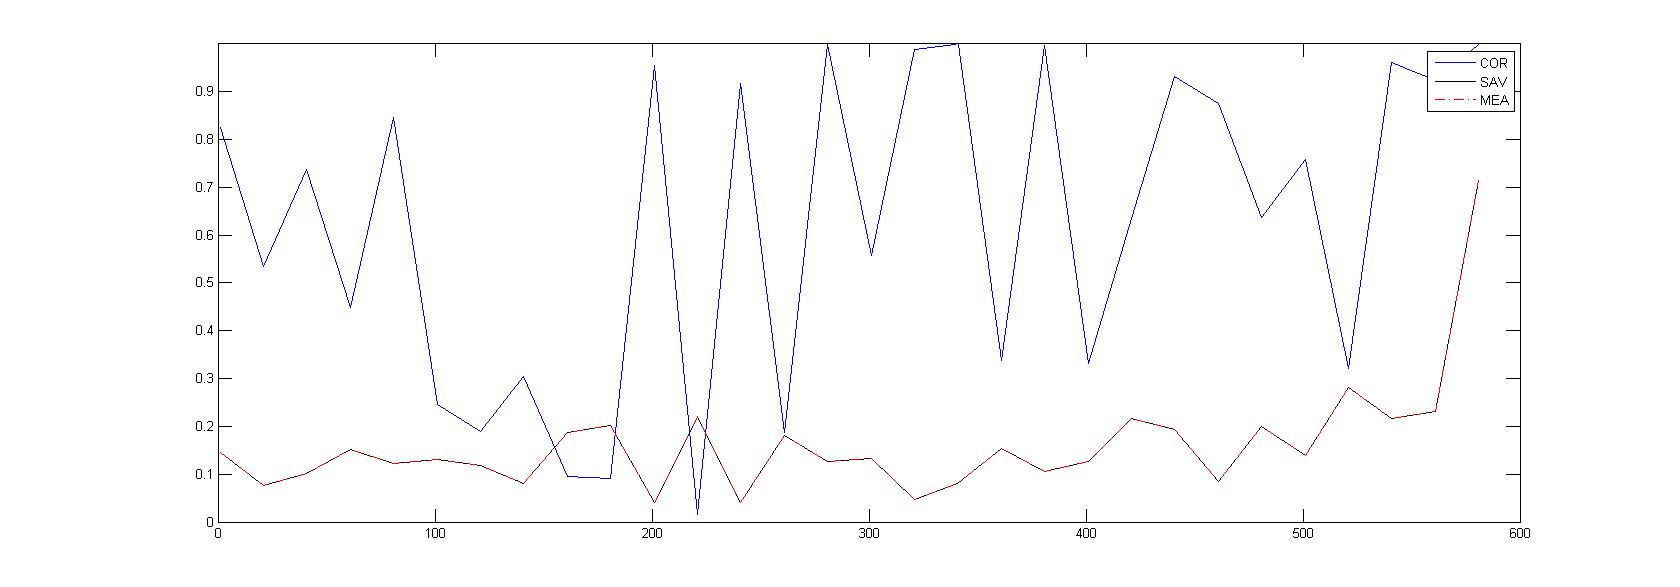
\includegraphics[width=\linewidth]{p_feature_group3}
\caption{The trends of various features in Group 3}
\end{figure}
From group 1, we select CON and VAR. From group 2 we select CLS and MAP. From group 3, we select COR and SAV. The feature selection results are listed in Table 3.26. We select 6 out of 16 feature parameters used in SVM, and achieve the classification accuracy of 70.33\% after assigning the RBF parameters with ($2^8$,$2^2$). 
\begin{table}[!b]
\centering
\renewcommand{\arraystretch}{0.5}
\begin{tabular}{|| c | c | c ||}
\hline
Index & Feature in Group & Selected Features \\
\hline
1 & Measures of Contrast & \\
  & CON, VAR, IDM,SVA, DVA, and DIS & CON and VAR \\
  \hline
2 & Measures of Uniformity & \\
  & ASM, SEN, ENT, CLS, CLP, and MAP & CLS and MAP \\
  \hline
3 & Measures of Correlation & \\
  & COR, SAV and MEA & COR and SAV \\
\hline
\end{tabular}
\caption{Feature selection sequence and the accuracy variation}
\end{table}
The result of comparison between two feature selection variables prove that combining two diffraction images can improve the representation of the diffraction image and help increase its pattern recognition accuracy. \par
By comparing most existing research in classification by using SVM, we discover that the accuracy level of 80.33\% is not good. In general, they can obtain the classification accuracy of over 90\%. For example, in Thati's research\cite{Thati}, the classification accuracy can reach 90\% when all texture features are applied and 89.83\% when features selected using the EFCS approach are applied. Furthermore, a study to detect fog using SVM obtains the high accuracy of 97.16\% for classification between foggy and non-foggy images\cite{Rakesh}. However, by comparing with the result using neural network for classification, SVM presents a high performance in classification. For instance, the wood defects classification using neural network achieves the accuracy of 78.26\%\cite{Qayyum}. The primary reason between the lower accuracy of our results is that the quality of our training data set is not good. As we mentioned before, all diffraction images are pre-classified manually based on people's experience. The accuracy cannot be guaranteed. In future research, the classification accuracy 80.33\% can be further improved by refining the training data set based on the results of SVM.  
\section{Conclusion}
During the empirical study, we applied texture features in SVM for classification. By applying 28 out of 34 texture features shown in Table 3.27, we obtained a classification accuracy of 80.33\%. To achieve this classification accuracy, we firstly performed a case study to select feature parameter. A feature parameter will be selected when it increases the classification accuracy of SVM. We started with a small training data set. After selecting seven feature parameters, we performed five-folder cross-validation on the classifier with the feature parameters we selected. The result revealed that we achieved an SVM classifier with an accuracy of 63.89\%, which is unstable and failed to generalize to new examples. To solve the problem, we obtained a new SVM classifier with an accuracy of 61.67\% using 11 feature parameters after we increased the size of the training data set to 2000. Nevertheless, the classification accuracy of 61.67\% is lower than the accuracy of the SVM classifier trained on the data with 32 feature parameters. The result showed a fact that some feature parameters which can be used in SVM were not examined. We obtained another SVM classifier by removing feature parameters which have a negative effect on classification accuracy. The classification accuracy of 65.67\% is the highest accuracy level achieved during the feature selection study. By performing the 10-folder cross-validation, we found the classifier to be stable. We further studied the improvement in the performance of SVM classifier. By modifying the parameter pair of (C, $\gamma$) in the RBF kernel, the classification accuracy of SVM can be affected. By examining various parameter pairs, we found the pair of ($2^{12}$, $2^{-3}$) to be the best. By applying the parameter pair in RBF kernel, the classification accuracy increased to 80.33\%. \par
Furthermore, we applied the EFCS approach from Thati's research for feature selection in the experiment. By selecting 2 uncorrelated feature parameters from each group, we obtain a classification accuracy of 70.33\% after modifying the parameter pair in the RBF kernel. The accuracy of 70.33\% is lower than we achieved. Thus, adding one more diffraction image can improve the representation of diffraction image. However, the classification accuracy we achieved is not as good. By comparing our results with some existing research, we discovered that our classification accuracy is much lower than theirs. The primary reason for the problem is that the training data we used for SVM are not classified correctly because of the complexity of the pattern recognition of the diffraction image. Nevertheless, the SVM algorithm has high performance in classification than neural network. We compared with other research using this algorithm and found some research obtained the accuracy which is lower than 80.33\%\cite{Qayyum}. Finally, if we consider the classification accuracy in selecting the valid diffraction images of Cell type, the SVM classifier has a high performance with the accuracy of 88.76\%.
Through the empirical study, we confirmed two diffraction images can improve their pattern recognition. We also validated that the SVM can be applied for image classification based on texture features of diffraction images. The parameters in the RBF kernel has a significant effect on classification accuracy. In comparison with other research using SVM, our classification accuracy is not good because the training data set we used needs to be further refined. However, in comparison with other research using the neural network in classification, our study presented a high performance in solving classification problems. 
\begin{table}[!t]
\begin{center}
\renewcommand{\arraystretch}{0.5}
\begin{tabular}{||c c c c c c c c||}
\hline
Index & Feature & Index & Feature & Index & Feature & Index & Feature\\[0.7ex]
\hline\hline
1 & s-ASM & 21 & p-ASM & 9 & s-ENT & 29 & p-ENT \\
2 & & 22 & p-CON & 10 & s-DEN & 30 & p-DEN \\
3 & s-COR & 23 & p-COR & 11 & s-DVA & 31 & p-DVA \\
4 & s-VAR & 24 & & 12 & s-DIS & 32 & p-DIS \\
5 & s-IDM & 25 & p-IDM & 13 & s-CLS & 33 & \\
6 & s-SAV & 26 & p-SAV & 14 & s-CLP & 34 & p-CLP \\
7 & s-SEN & 27 & p-SEN & 16 & s-MAP & 36 & \\
8 & s-SVA & 28 & p-SVA & 17 & s-MEA & 37 & p-MEA \\
\hline
\end{tabular}
\caption {The 28 texture features applied in SVM for classification}
\end{center}
\end{table}
    